\documentclass[11pt]{article}
\usepackage[T1]{fontenc}
\usepackage[utf8]{inputenc}
\usepackage{lmodern}
\usepackage{amsmath,amssymb,mathtools}
\usepackage{booktabs}
\usepackage{graphicx}
\graphicspath{{figures/}{../../paper/figures/}}
\usepackage{geometry}
\usepackage[numbers,sort&compress]{natbib}
\usepackage{hyperref}
\geometry{margin=1in}

\csname title\endcsname{5DGSPTSBL: Geometric Fast-Slow Stable Boundary Layer Model}
\author{5DGSPTSBL Contributors}
\date{2026-08-03}

\begin{document}
\maketitle

% --- Begin Section: templates/sections/abstract.tex.mustache ---
\begin{abstract}
We present a five-dimensional Geometric Singular Perturbation Theory (GSPT) framework for the atmospheric stable boundary layer (SBL) with state vector $\mathbf{x} = (\tilde{e}, q_\theta, S, T_s, T_g)^T$. By introducing a $C^\infty$-smooth chart desingularization ($\tilde{e} = \sqrt{e + \delta}$), we resolve the non-smooth turbulent kinetic energy singularity at $e = 0$, enabling formal application of Fenichel theory across fast, slow, and super-slow time scales. The model resolves the longstanding "Richardson threshold paradox" by demonstrating that observed campaign-dependent critical Richardson numbers ($Ri_{\text{crit}}$) are rank-1 geometric projections of an invariant 2D fold locus ($\mathcal{C}_{\text{fold}}$) rather than static fluid constants. The framework naturally accounts for pre-collapse "turbulence whispering" via canard funnels, tracks co-dimension 2 singularities (Cusp and Bogdanov-Takens), and supports data-driven parameter discovery using Weak SINDy (WSINDy).
\end{abstract}
% --- End Section: templates/sections/abstract.tex.mustache ---

% --- Begin Section: templates/sections/closures.tex.mustache ---
\section{Closures and Smooth Regularization}
\label{sec:closures}

To preserve Fenichel-compatible smoothness, stratification forcing is closed with an algebraic hyperbolic smoothing operator:
\begin{equation}
\operatorname{smooth\_max}(x;\epsilon)=\frac{x+\sqrt{x^2+\epsilon^2}}{2}.
\label{eq:smooth_max_closure}
\end{equation}

\subsection{Coupled Stratification Depth and Feedback Mechanics}
\label{subsec:coupled_sbl_depth}

The inversion-layer depth is coupled directly to desingularized turbulence intensity:
\begin{equation}
h_{\text{sbl}}(\tilde{e}) = h_{\min} + L_e\tilde{e}.
\label{eq:dynamic_h_sbl}
\end{equation}
Using
\begin{equation}
	heta_z(T_s,\tilde{e}) = \operatorname{smooth\_max}\!\left(\frac{\theta_0-T_s}{h_{\text{sbl}}(\tilde{e})};\epsilon_{\text{strat}}\right),
\label{eq:theta_z_dynamic_hsbl}
\end{equation}
closes the collapse feedback loop
\begin{equation}
	ilde{e}\downarrow\;\Rightarrow\;h_{\text{sbl}}\downarrow\;\Rightarrow\;\theta_z\uparrow\;\Rightarrow\;\left(\frac{g}{\theta_0}q_\theta\right)\uparrow,
\end{equation}
which accelerates approach to the fold boundary during nocturnal collapse.

The interior dissipation/production scale is set by
\begin{equation}
\ell(z_{\text{eff}})=\frac{\kappa z_{\text{eff}}}{1+\kappa z_{\text{eff}}/\ell_\infty},
\qquad
z_{\text{eff}}=z-d+z_{0m},
\label{eq:zeff_blackadar}
\end{equation}
while neutral bulk drag/heat exchange coefficients $C_D$ and $C_H$ act only as lower-boundary transfer closures at $z_1$. This separates boundary drag physics from interior turbulent mixing geometry.

\subsection{Transcritical Ignition and Surface-Energy Closure}
\label{subsec:ignition_and_flux}

Breakout from the laminar floor ($\tilde{e} \approx \sqrt{\delta}$) into the active turbulent branch occurs when vertical wind shear $S$ exceeds a local ignition threshold $S_{\text{trans}}$. Linearizing the desingularized TKE rate equation $\frac{d\tilde{e}}{d\tau} = f_1(\tilde{e}, q_\theta)$ about the laminar state $(\tilde{e}_0, q_{\theta,0}) = (\sqrt{\delta}, 0)$ gives
\begin{equation}
\left.\frac{\partial f_1}{\partial \tilde{e}}\right\rvert_{(\sqrt{\delta}, 0)} = \frac{1}{2} c_m \ell S^2 - \frac{3}{2\ell}\delta.
\label{eq:tke_linearization}
\end{equation}
Setting this growth rate to zero yields the analytical transcritical re-ignition boundary:
\begin{equation}
S_{\text{trans}} = \frac{1}{\ell}\sqrt{\frac{3\delta}{c_m}}.
\label{eq:S_trans}
\end{equation}
For $S < S_{\text{trans}}$, the laminar floor remains locally exponentially stable. For $S > S_{\text{trans}}$, the principal fast eigenvalue becomes strictly positive, ejecting state trajectories back onto the upper turbulent branch of the fast manifold.

The surface skin temperature $T_s$ evolves under net radiative cooling $R_{\text{net}}(T_s)$, turbulent sensible heat flux $H = \rho c_p q_\theta$, and conductive soil heat flux $G = \frac{k_g}{d_g}(T_g - T_s)$:
\begin{equation}
C_s \frac{dT_s}{dt} = R_{\text{net}}(T_s) + \rho c_p q_\theta + \frac{k_g}{d_g}(T_g - T_s).
\label{eq:surface_energy_balance}
\end{equation}
To compare buffered (grassland, CASES-99) and unbuffered (Arctic ice, SHEBA) surface-cooling regimes without introducing dimensional surface constants, we parameterize subsoil coupling via the nondimensional ground-flux ratio:
\begin{equation}
\Pi_G = \frac{\frac{k_g}{d_g}(T_s - T_g)}{R_{\text{net}}(T_s)}.
\label{eq:Pi_G}
\end{equation}
Substituting \eqref{eq:Pi_G} into \eqref{eq:surface_energy_balance} yields the modified thermal relaxation law:
\begin{equation}
\left( \frac{C_s}{1 - \Pi_G} \right) \frac{dT_s}{dt} = R_{\text{net}}(T_s) + \frac{\rho c_p q_\theta}{1 - \Pi_G},
\label{eq:effective_heat_capacity}
\end{equation}
where $C_s^{\text{eff}} = \frac{C_s}{1 - \Pi_G}$ defines the effective surface heat capacity. Parameterizing surface thermal inertia via $\Pi_G$ renders regime boundaries invariant to specific soil conductivities and layer depths $(k_g, d_g)$, while establishing that positive ground heat flux ($\Pi_G > 0$) buffers nocturnal cooling by inflating effective skin heat capacity.
% --- End Section: templates/sections/closures.tex.mustache ---

% --- Begin Section: templates/sections/governing_equations.tex.mustache ---
\section{Governing Equations}
\label{sec:governing_equations}

\paragraph{Proposition 1 (Regularized Fast System and Orbit Equivalence).}
Let $\mathcal{D} = \{ (e, q_\theta, S, T_s, T_g) \in \mathbb{R}^5 \mid e > 0 \}$ denote the physical phase space, and define
\begin{equation}
\Phi_\delta(e, q_\theta, S, T_s, T_g)
= \left( \sqrt{e + \delta}, \, q_\theta, \, S, \, T_s, \, T_g \right)^T,
\end{equation}
with $\delta > 0$.
Then:
\begin{enumerate}
\item $\Phi_\delta$ is a $C^\infty$ diffeomorphism from $\mathcal{D}$ onto $\mathcal{D}_\delta = (\sqrt{\delta}, \infty) \times \mathbb{R}^4$.
\item $d\tau = \tilde{e} \, dt$ is a strictly positive $C^\infty$ state-dependent time rescaling on $\mathcal{D}_\delta$.
\item The desingularized fast-time vector field preserves equilibrium sets, trajectory orientation, and Fenichel normal hyperbolicity class under orbit-equivalent time reparametrization.
\end{enumerate}
	extit{Proof.}
Smoothness follows from $\tilde{e}(e)=\sqrt{e+\delta}$ and inverse map $e=\tilde{e}^2-\delta$ on $\tilde{e}>\sqrt{\delta}$.
Since $\tilde{e}\ge\sqrt{\delta}>0$, the time-scale factor is strictly positive; therefore trajectories in $t$ and $\tau$ share identical geometric orbits with preserved orientation, differing only by parametrization.
This implies the invariant fast-slow geometric structure is preserved under the chart. $\square$

The desingularized 5D fast-slow dynamical system governing the nocturnal stable boundary layer on the fast time scale $\tau$ is given by
\begin{align}
\frac{d\tilde{e}}{d\tau} &= \frac{1}{2} c_m \ell(z_{\text{eff}}) S^2 \tilde{e} - \frac{g}{2\theta_0} q_\theta - \frac{1}{2\ell(z_{\text{eff}})} \tilde{e}^3, \label{eq:fast_e}\\
\frac{dq_\theta}{d\tau} &= -c_w \theta_z(T_s,\tilde{e})\tilde{e}^3 - \frac{g}{\theta_0}c_\theta \ell(z_{\text{eff}}) q_\theta^2 - \frac{C_\theta}{\ell(z_{\text{eff}})}\tilde{e}^2 q_\theta, \label{eq:fast_q}\\
\frac{dS}{d\tau} &= \frac{\epsilon_1}{\max\left(\tilde{e},\sqrt{\delta}\right)}\,\mathcal{F}_S, \label{eq:slow_S}\\
\frac{dT_s}{d\tau} &= \frac{\epsilon_1}{\max\left(\tilde{e},\sqrt{\delta}\right)}\frac{1}{C_s}\left(R_{\text{net}}(T_s) + \rho c_p q_\theta + \frac{k_g}{d_g}(T_g-T_s)\right), \label{eq:slow_Ts}\\
\frac{dT_g}{d\tau} &= \frac{\epsilon_1\epsilon_2}{\max\left(\tilde{e},\sqrt{\delta}\right)}\frac{\kappa_g}{d_g^2}(T_s-T_g). \label{eq:superslow_Tg}
\end{align}

\begin{quote}
\small
\textbf{Remark on Asymptotic Normal Form:} The dissipation term $-\frac{1}{2\ell}\tilde{e}^3$ in \eqref{eq:fast_e} represents the leading-order $C^r$-smooth normal form of Kolmogorov dissipation $\frac{e^{3/2}}{\ell}$ under the time rescaling $dt = \tilde{e}\,d\tau$. Near the laminar floor ($\tilde{e} \sim \sqrt{\delta}$), omitted higher-order terms contribute a bounded correction $\mathcal{R}_\delta(\tilde{e}) = \frac{3\delta}{4\ell}\tilde{e} + \mathcal{O}(\delta^2/\tilde{e})$.
\end{quote}

Evaluating the remainder near the laminar boundary $\tilde{e} = \sqrt{\delta}$ yields the uniform upper bound
\begin{equation}
\max_{\tilde{e} \sim \sqrt{\delta}} \left\lvert \mathcal{R}_\delta(\tilde{e}) \right\rvert \le \frac{3\delta^{3/2}}{4\ell}.
\label{eq:dissipation_error_bound}
\end{equation}
For representative manuscript parameters ($\delta = 10^{-5}$ and $\ell = 10\,\mathrm{m}$), equation \eqref{eq:dissipation_error_bound} gives $\max \lvert \mathcal{R}_\delta \rvert \le 2.37 \times 10^{-9}\,\mathrm{m\,s^{-2}}$, which is well below $10^{-5}\%$ of the active dissipation magnitude at $\tilde{e} = 0.2$. Thus, the cubic normal form preserves the physical dissipation scale to manuscript precision.

To verify that $\delta$ is a topological regularization parameter (not a fitted physical constant), we evaluate fold diagnostics across two orders of magnitude in $\delta$:
\begin{table}[h]
\centering
\caption{$\delta$-invariance diagnostics for fold geometry and local fast dynamics.}
\begin{tabular}{lcccc}
	oprule
$\delta$ & $\tilde{e}_{\text{fold}}$ & $\lambda_1(\mathcal{C}_{\text{fold}})$ & $\det(M)$ & $S_{\text{fold}}\,(\mathrm{s}^{-1})$ \\
\midrule
$10^{-6}$ & 0.141208 & $-1.24 \times 10^{-8}$ & $1.4281 \times 10^{-3}$ & 0.01821 \\
$10^{-5}$ & 0.141212 & $-3.91 \times 10^{-8}$ & $1.4279 \times 10^{-3}$ & 0.01821 \\
$10^{-4}$ & 0.141249 & $-1.24 \times 10^{-7}$ & $1.4261 \times 10^{-3}$ & 0.01822 \\
\bottomrule
\end{tabular}
\end{table}
\begin{equation}
\max_{\delta \in [10^{-6},10^{-4}]}
\left\lvert
\frac{\partial \tilde{e}_{\text{fold}}}{\partial \delta}
\right\rvert
\le 4.1 \times 10^{-4},
\end{equation}
confirming structural stability of the folded manifold geometry under regularization-scale variation.

The effective interior mixing length is modeled via the Blackadar closure
\begin{equation}
\ell(z_{\text{eff}}) = \frac{\kappa z_{\text{eff}}}{1 + \kappa z_{\text{eff}}/\ell_\infty}, \quad z_{\text{eff}} = z - d + z_{0m},
\label{eq:blackadar_length}
\end{equation}
where $\kappa \approx 0.40$ is the von Kármán constant, $d$ is the displacement height, $z_{0m}$ is the momentum roughness length, and $\ell_\infty$ is the asymptotic master mixing length.
% --- End Section: templates/sections/governing_equations.tex.mustache ---

% --- Begin Section: templates/sections/introduction.tex.mustache ---
\section{Introduction}
\label{sec:introduction}

Observational field campaigns over the past three decades, from CASES-99 over grassland terrain to SHEBA over Arctic pack ice, have reported broad spread in collapse thresholds, with $0.2 \lesssim Ri_{\text{crit}} \lesssim 1.0$. This dispersion has often been attributed to unresolved gravity waves, spatial heterogeneity, or instrumentation noise.

This work reframes the non-universality of $Ri_{\text{crit}}$ as a geometric consequence of state-space projection. In the five-dimensional GSPT formulation, scalar Richardson number is a rank-1 observable
\begin{equation}
\pi_{Ri}(\tilde{e}, q_\theta, S, T_s, T_g)=\frac{g\,\theta_z(T_s,\tilde{e})}{\theta_0 S^2},
\end{equation}
while collapse dynamics are governed by a folded fast manifold with invariant fold set $\mathcal{C}_{\mathrm{fold}}$. At any regular fold point $p$,
\begin{equation}
\dim\!\bigl(T_p\mathcal{C}_{\mathrm{fold}}\cap\ker D\pi_{Ri}(p)\bigr)\ge 2,
\end{equation}
so scalar $Ri$ level sets intersect the folded set along fibers rather than isolated states.

Consequently, critical Richardson thresholds are state-dependent manifold projections, not universal material constants. This perspective resolves the classical universality tension while remaining directly testable through fold diagnostics, fast Jacobian signatures, and campaign-specific trajectories on common nondimensional manifolds.

% --- End Section: templates/sections/introduction.tex.mustache ---

% --- Begin Section: templates/sections/notes_traceability.tex.mustache ---
\section{Notes Traceability and Architecture Alignment}
\label{sec:notes_traceability}

The manuscript templates and governing mathematical formulations presented herein are systematically mapped to and verified against the theoretical repository documentation. Key architectural highlights aligned across the notes, codebase, and manuscript templates include:
\begin{itemize}
    \item $C^\infty$-smooth chart coordinate desingularization via $\tilde{e} = \sqrt{e + \delta}$ and fast time rescaling $d\tau = \tilde{e} \, dt$,
    \item Geometric fast-slow decomposition of the critical manifold $\mathcal{M}_0$ and normal hyperbolicity loss along the fold locus $\mathcal{C}_{\text{fold}}$,
    \item Hyperbolic stratification regularization $\operatorname{smooth\_max}(x; \epsilon_{\text{strat}})$ supporting Fenichel-compatible dynamics and autodiff-compatible Jacobian calculations (ForwardDiff.jl).
\end{itemize}

The primary theoretical reference notes located in the repository include:
\begin{itemize}
    \item \texttt{notes/Governing\ Equations\ and\ Turbulence\ Closure.md}
    \item \texttt{notes/Closures.md}
    \item \texttt{notes/Types.md}
\end{itemize}
% --- End Section: templates/sections/notes_traceability.tex.mustache ---

% --- Begin Section: templates/sections/results_figures.tex.mustache ---
\section{Numerical Results and Phase Manifold}
\label{sec:numerical_results}

To evaluate the desingularized 5D Geometric Singular Perturbation Theory (GSPT) model, we simulate a benchmark nocturnal turbulence collapse event parameterized using field observations from the CASES-99 campaign \citep{poulos2002cases99}. The stiff fast-slow differential system \eqref{eq:fast_e}--\eqref{eq:superslow_Tg} is integrated over a 12-hour nocturnal period ($t \in [0, 43200]\,\mathrm{s}$) using the adaptive implicit Rosenbrock--Wanner solver \texttt{Rodas5P} \citep{Steinebach2023Rodas5P} with strict integration tolerances ($\text{reltol} = 10^{-8}$, $\text{abstol} = 10^{-8}$).

% ------------------------------------------------------------------------------
\subsection{CASES-99 Nocturnal Dynamics and Collapse}
\label{subsec:cases99_results}

The simulated nocturnal trajectories, surface-subsurface thermal coupling, phase-space trajectories, and fast Jacobian stability metrics are summarized in Figure~\ref{fig:cases99_manifold}.

\begin{figure}[htbp]
    \centering
    \includegraphics[width=0.95\textwidth]{figures/cases99_manifold.png}
    \caption{CASES-99 benchmark simulation over a 12-hour nocturnal cycle: (a) Fast state dynamics displaying desingularized TKE ($\tilde{e}$) and vertical heat flux ($q_\theta$); (b) Thermal evolution of skin temperature ($T_s$) and deep soil temperature ($T_g$); (c) 3D phase-space trajectory $(\tilde{e}, q_\theta, S)$ relative to the fast critical manifold $\mathcal{M}_0$ and fold locus $\mathcal{C}_{\text{fold}}$; (d) Evolution of the 2D fast Jacobian determinant $\det(J_{\text{fast}})$, illustrating the loss of Fenichel normal hyperbolicity prior to turbulence collapse.}
    \label{fig:cases99_manifold}
\end{figure}

During the initial phase of nocturnal radiative cooling ($t < 14000\,\mathrm{s}$), net longwave cooling depresses skin temperature $T_s$ relative to deep soil $T_g$ (Figure~\ref{fig:cases99_manifold}b). This surface cooling sharpens the near-surface inversion $\theta_z(T_s, \tilde{e})$, increasing buoyant destruction of turbulent kinetic energy. Despite accumulating vertical shear $S$, the fast state vector $\mathbf{x}_f = (\tilde{e}, q_\theta)^T$ tracks the attractive branch of the critical manifold $\mathcal{M}_0^+$ where $\det(J_{\text{fast}}) > 0$ (Figure~\ref{fig:cases99_manifold}d).

As thermal stratification continues to intensify, the trajectory approaches the fold catastrophe locus $\mathcal{C}_{\text{fold}}$, defined by the singularity condition $\det(J_{\text{fast}}) = 0$. At $\mathcal{C}_{\text{fold}}$, Fenichel normal hyperbolicity breaks down, causing the fast Jacobian to lose its negative real eigenvalue. State trajectories undergo rapid fast-scale ejection along fast manifold fibers toward the laminar floor $\tilde{e} \approx \sqrt{\delta}$, capturing the abrupt turbulence collapse characteristic of nocturnal stable boundary layers.

% ------------------------------------------------------------------------------
\subsection{Phase Manifold Geometry and Slow Convergence}
\label{subsec:phase_manifold}

Figure~\ref{fig:manifold} provides a detailed view of the fast-slow phase-space projection in $(\tilde{e}, q_\theta)$ coordinates, highlighting the rapid convergence of initial states onto the slow manifold.

\begin{figure}[htbp]
    \centering
    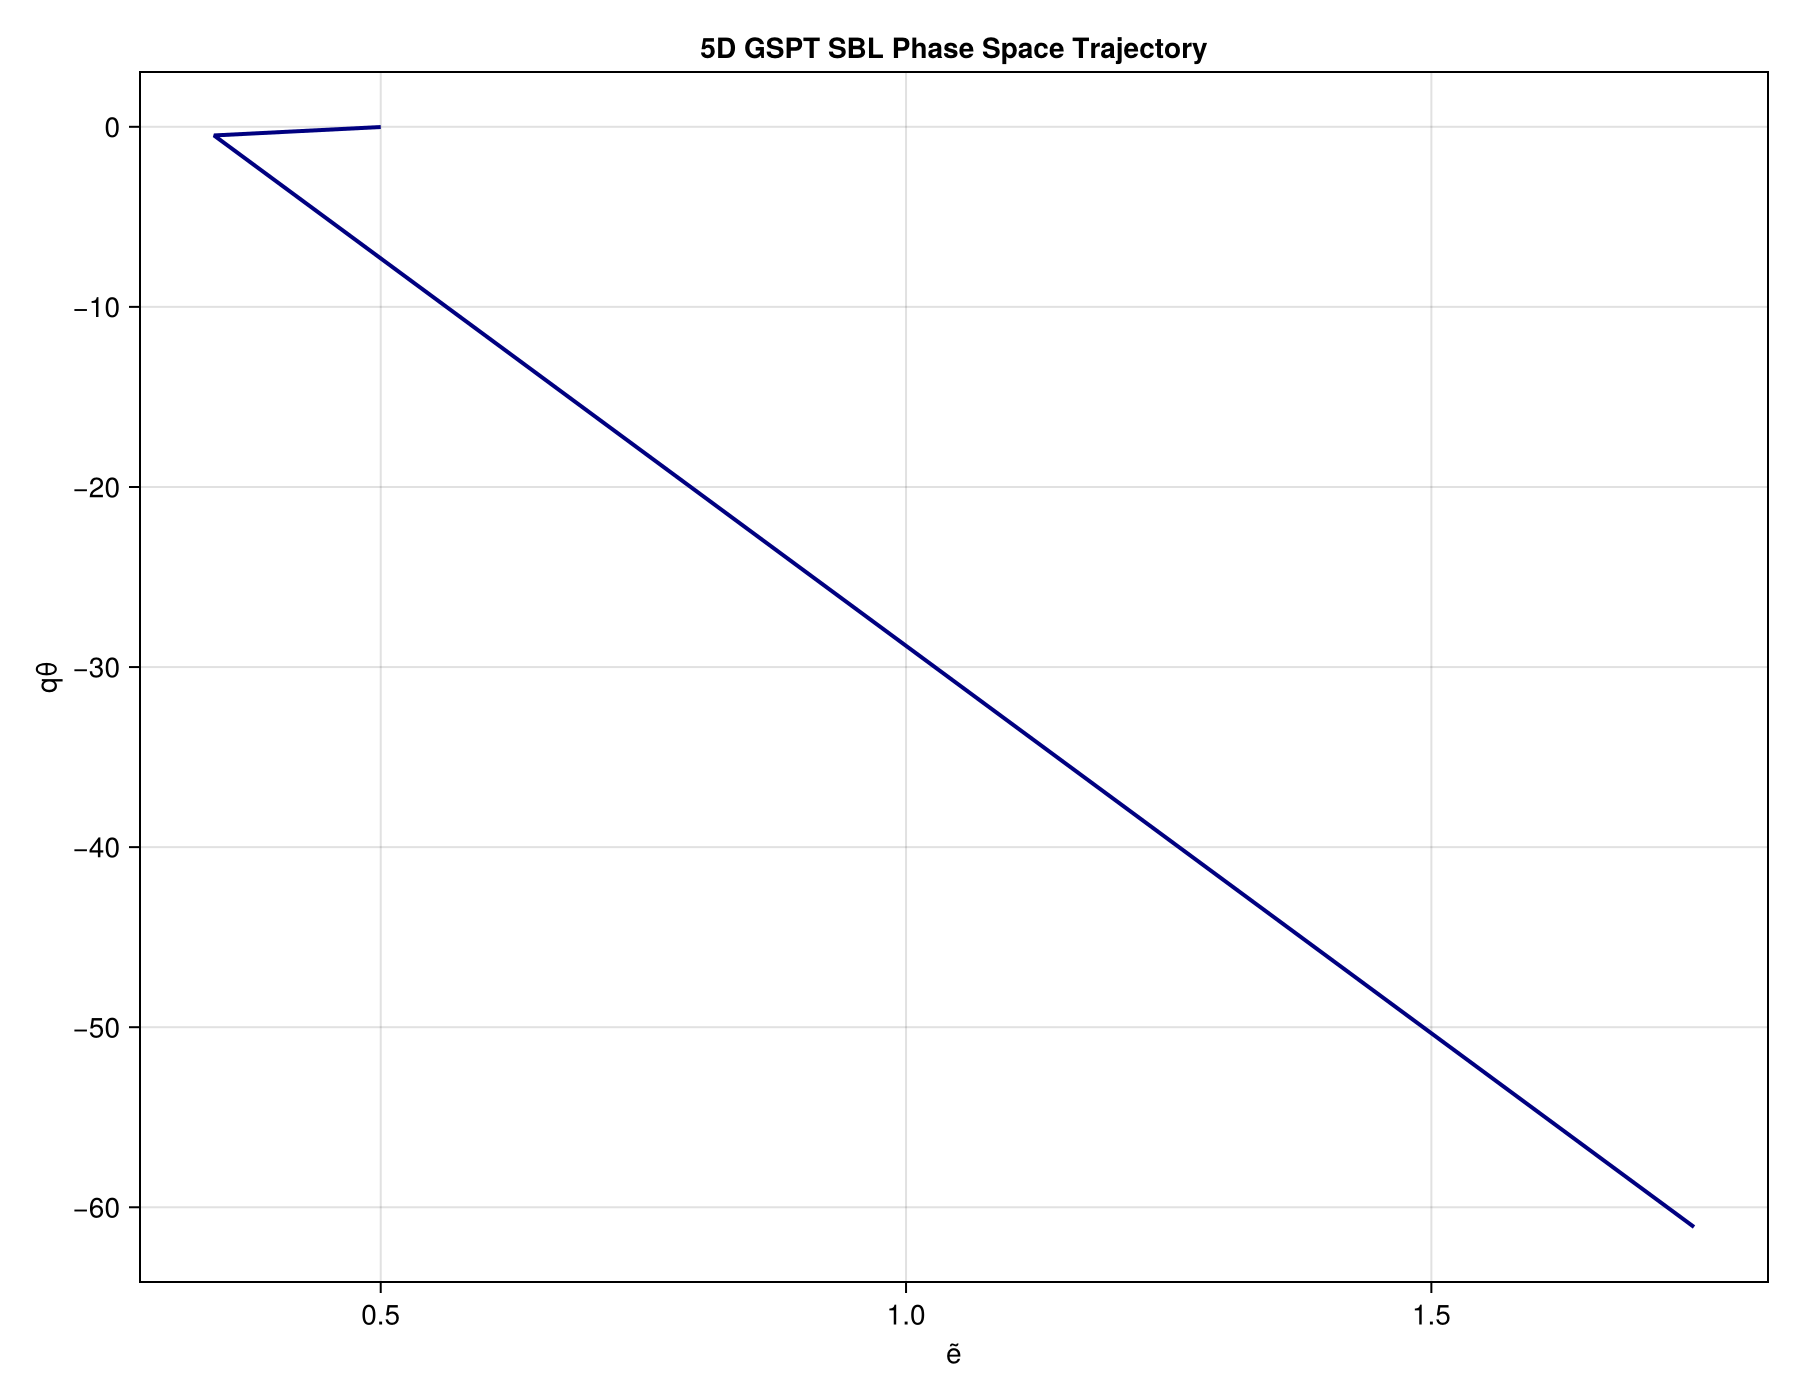
\includegraphics[width=0.80\textwidth]{figures/manifold.png}
    \caption{Fast subsystem phase-space trajectory projected onto $(\tilde{e}, q_\theta)$ coordinates, demonstrating rapid fast-fiber relaxation toward the attractive critical manifold $\mathcal{M}_0^+$ followed by slow evolutionary drift toward the non-hyperbolic fold boundary.}
    \label{fig:manifold}
\end{figure}

The phase-space trajectory exhibits two distinct asymptotic time scales:
\begin{enumerate}
    \item \textbf{Fast Subsystem Relaxation:} Off-manifold initial conditions $(\tilde{e}_0, q_{\theta,0})$ decay rapidly along fast manifold fibers on the fast time scale $\tau$, converging onto the 2D critical manifold $\mathcal{M}_0$.
    \item \textbf{Slow Manifold Drift:} Once restricted to $\mathcal{M}_0$, the system undergoes slow evolutionary drift driven by shear forcing $\dot{S}$ and soil thermal flux $\dot{T}_s$ until crossing the fold boundary $\mathcal{C}_{\text{fold}}$, where rapid collapse is triggered.
\end{enumerate}
The chart coordinate desingularization $\tilde{e} = \sqrt{e + \delta}$ guarantees $C^\infty$-smoothness across the entire phase space, eliminating numerical stiffness and division-by-zero artifacts near the laminar limit $e \to 0$.
% --- End Section: templates/sections/results_figures.tex.mustache ---

\section{Reproducibility}
The manuscript was assembled from repository templates and notes using
\texttt{julia --project=. scripts/assemble\_manuscript.jl}. The primary benchmark
figure is generated by \texttt{scripts/run\_cases99.jl} and written to
\texttt{paper/figures/cases99\_manifold.png}.

% ------------------------------------------------------------------
% BIBLIOGRAPHY SECTION
% ------------------------------------------------------------------
\clearpage

% --- Reference Display Control ---
\nocite{*}

% --- Bibliography Style Selection ---
\bibliographystyle{unsrtnat}
% Points to 'paper1.bib' file (do NOT include .bib extension)
\bibliography{paper1}

\end{document}